%\title{SlugCam submission for PerCom 2015}
%% percomPaper.tex
%% Draft version: 1.0
%% 8/25/2014
%% Authors:
%% Kevin Abas
%% Leland Miller
%% Katia Obraczka
%% see SlugCam's Organization page: https://github.com/SlugCam



%%*************************************************************************
%% Legal Notice:
%% This code is offered as-is without any warranty either expressed or
%% implied; without even the implied warranty of MERCHANTABILITY or
%% FITNESS FOR A PARTICULAR PURPOSE! 
%% User assumes all risk.
%% In no event shall IEEE or any contributor to this code be liable for
%% any damages or losses, including, but not limited to, incidental,
%% consequential, or any other damages, resulting from the use or misuse
%% of any information contained here.
%%
%% All comments are the opinions of their respective authors and are not
%% necessarily endorsed by the IEEE.
%%
%% This work is distributed under the LaTeX Project Public License (LPPL)
%% ( http://www.latex-project.org/ ) version 1.3, and may be freely used,
%% distributed and modified. A copy of the LPPL, version 1.3, is included
%% in the base LaTeX documentation of all distributions of LaTeX released
%% 2003/12/01 or later.
%% Retain all contribution notices and credits.
%% ** Modified files should be clearly indicated as such, including  **
%% ** renaming them and changing author support contact information. **
%%
%% File list of work: IEEEtran.cls, IEEEtran_HOWTO.pdf, bare_adv.tex,
%%                    bare_conf.tex, bare_jrnl.tex, bare_jrnl_compsoc.tex,
%%                    bare_jrnl_transmag.tex
%%*************************************************************************


%
\documentclass[10pt,conference]{IEEEtran}
%



% Some very useful LaTeX packages include:
% (uncomment the ones you want to load)


% *** MISC UTILITY PACKAGES ***
%
%\usepackage{ifpdf}
%
% \ifpdf
%   % pdf code
% \else
%   % dvi code
% \fi


% *** CITATION PACKAGES ***
%
%\usepackage{cite}


% *** GRAPHICS RELATED PACKAGES ***
%
\ifCLASSINFOpdf
  % \usepackage[pdftex]{graphicx}
  % declare the path(s) where your graphic files are
  % \graphicspath{{../pdf/}{../jpeg/}}
  % and their extensions so you won't have to specify these with
  % every instance of \includegraphics
  % \DeclareGraphicsExtensions{.pdf,.jpeg,.png}
\else
  % or other class option (dvipsone, dvipdf, if not using dvips). graphicx
  % will default to the driver specified in the system graphics.cfg if no
  % driver is specified.
  % \usepackage[dvips]{graphicx}
  % declare the path(s) where your graphic files are
  % \graphicspath{{../eps/}}
  % and their extensions so you won't have to specify these with
  % every instance of \includegraphics
  % \DeclareGraphicsExtensions{.eps}
\fi


% *** MATH PACKAGES ***
%
%\usepackage[cmex10]{amsmath}


% *** SPECIALIZED LIST PACKAGES ***
%
%\usepackage{algorithmic}


% *** ALIGNMENT PACKAGES ***
%
%\usepackage{array}


% *** SUBFIGURE PACKAGES ***
%\ifCLASSOPTIONcompsoc
%  \usepackage[caption=false,font=normalsize,labelfont=sf,textfont=sf]{subfig}
%\else
%  \usepackage[caption=false,font=footnotesize]{subfig}
%\fi


% *** FLOAT PACKAGES ***
%
%\usepackage{fixltx2e}
%
%\usepackage{stfloats}
%
%\usepackage{dblfloatfix}
%
%\ifCLASSOPTIONcaptionsoff
%  \usepackage[nomarkers]{endfloat}
% \let\MYoriglatexcaption\caption
% \renewcommand{\caption}[2][\relax]{\MYoriglatexcaption[#2]{#2}}
%\fi
%
% For subfig.sty:
% \let\MYorigsubfloat\subfloat
% \renewcommand{\subfloat}[2][\relax]{\MYorigsubfloat[]{#2}}
%

%Figure Package
\usepackage{graphicx}

% *** PDF, URL AND HYPERLINK PACKAGES ***
%
\usepackage{url}


\begin{document}


%% ***********************  THE TITLE **********************************



\title{Solar-Powered Smart Wireless Camera Network for Ubiquitous Outdoor Monitoring}



%% ***********************  AUTHORS ************************************



\author{\IEEEauthorblockN{Kevin Abas\IEEEauthorrefmark{1},
Leland Miller \IEEEauthorrefmark{1},
Katia Obraczka\IEEEauthorrefmark{1}}
\IEEEauthorblockA{\IEEEauthorrefmark{1}School of Engineering,
University of California Santa Cruz, CA 95064 USA}
}



%% ***********************  Abstract ************************************



\IEEEtitleabstractindextext{%
\begin{abstract}

In this paper, we present SlugCam, a solar-powered wireless smart camera network platform that can be used in a variety of outdoor applications including surveillance of public spaces, habitat and environmental monitoring, wildfire prevention and detection, to name a few. SlugCam was designed such that it can be deployed and left unattended for extended periods without requiring regular maintenance, e.g., frequent battery replacement. The system is built with off-the-shelf components which not only keeps it modular and low cost, but also facilitates its prototyping, reproducibility, and evolution.  SlugCam’s onboard processing capability allows computer vision software to run locally which contributes to the system’s autonomous operation capabilities. Energy efficiency in SlugCam is accomplished both in hardware by using low-power components and software.  The system’s duty cycles automatically adapt to the current state of the battery in order to balance the trade-off between application-level requirements and power awareness. For instance, SlugCam’s smart camera changes its monitoring behavior based on how much battery charge remains. Additionally, using its computer vision software, the system only records and transmits information upon event detection which contributes both to the system’s energy efficiency as well as its low network bandwidth requirements. Another important contribution of SlugCam is to provide an open-source network software platform that can adapt to future requirements of a variety of visual sensor networks and their applications. For example, SlugCam’s user interface software maps and tags events to the corresponding video footage captured by camera nodes in order to present collections of fragmented information in a cohesive manner. In addition to a detailed description of SlugCam, this paper presents an extensive power characterization of the system’s operation and showcases its deployment in a real-world scenario. 

\end{abstract}

}

%% ********************** IEEE KEYWORDS ********************************



%\begin{IEEEkeywords}
%Real-time systems and embedded
%systems,Interactive systems, Web services, visual sensor networks
%\end{IEEEkeywords}


% make the title area
\maketitle

\IEEEdisplaynontitleabstractindextext
% \IEEEdisplaynontitleabstractindextext has no effect when using
% compsoc or transmag under a non-conference mode.

% For peerreview papers, this IEEEtran command inserts a page break and
% creates the second title. It will be ignored for other modes.
\IEEEpeerreviewmaketitle



%%
%% *********************  BEGIN PAPER **********************************
%%



\section{Introduction}


 \IEEEPARstart{I}{}ntroduction here discussing the paper
 Bring up both areas we'll be discussing 



%%
%% *********************  Section 2 **********************************
%%



\section{Motivation}

Explain campus safety application possibly? Potential use cases




%%
%% *********************  Section 3 **********************************
%%



\section{System Overview}

SlugCam has been designed with readily available devices  to reduce cost and to allow for rapid development. Due to our low powered solar capabilities, each sub-component has been chosen carefully to meet our power consumption efficiency requirements . We've designed the system to have better video processing capabilities than previously designed smart cameras \cite{SWEETcam}. Knowing that this would require us to balance the power consumed, we have made SlugCam extremely adaptive to the available energy remaining in the rechargeable battery. Combine the previous two features with the systems ability to be more selective of the video it records and we believe we have balanced accuracy, energy, and bandwidth efficiency as is demanded by smart camera networks \cite{AccLatEnergy}. Having difficulties finding software that suited our needs for viewing the video sensor data, we have also designed open-source camera node and sensor data management software. Although we're currently using just using a passive infrared sensor, many other sensors could be added to any of the available I/O ports, allowing the node to adapt to different application requirements. 
	
    \subsection{Power Adaptability of Hardware}

Our platform makes use of the widely used MSP430 microprocessor to act as the embedded system controller \cite{msp430}. The MSP430 is lower powered and it can put itself into 4 different low powered sleep states. SlugCam's Main processing device is the Raspberry Pi \cite{raspberrypi} which runs the nodes main tasks and the computer vision software. Having the MSP430 power the Raspberry Pi only when necessary makes the system able to adapt its power consumption use. Every external module used including the PIR, camera, and WiFi modules have the ability to be powered down as well, so the system's normal routines can be changed based on what energy amount is available. SlugCam can then alternate its power consuming states by changing its defined duty cycles. 

	\subsection{Outdoor Deployment}

As previously mentioned, one of SlugCam's main goal when first designed was its ability to not rely on the power grid and to be remotely deployed. Using Directional WiFi antennas SlugCam is completely wireless and can be deployed in areas with readily available sunlight, but very little ability of accessing the power grid. In fact the system never needs to be serviced for batteries as many wireless sensor network devices require. Solar technologies costs have reduced to make this a very viable power resource to researchers and why we have designed it in SlugCam. With its ability to run processing extensive tasks on board, SlugCam can run autonomously without the need of a centralized network coordinator. Unlike systems which offload large amounts of video footage to a more powerful webservers, SlugCam does image processing locally and is more selective about the data it transmits. Lowering the data needing to be transmitted assists the system in being bandwidth efficient in this outdoor scenarios where wireless communication isn't as fast as their wired counterparts. Smarter off-grid autonomous monitoring devices like SlugCam allow for endless application possibilities.
	
	\subsection{Open-Source and extensibility}
Modularity of components
Allows for ease of extending system
Allows developers to approach code in a way that is easy to understand
Each device has been isolated for its functionality and is considered when the device needs to adapt to power consumption needs
Sensors can be added and customized for specific applications

	\subsection{Designing a platform and a user interface}
Not only does the SlugCam project support a smart camera platform, but we've also designed a webserver stack and an innovative user interface for managing the Captured data. Users will also be able to track, query, and configure their SlugCam nodes using the provided apps and server software. We later describe the importance of the software and go into futher detail about how it plays a role in the SlugCam system.



%%
%% *********************  Section 4 **********************************
%%

\begin{figure}[h!]
\centering
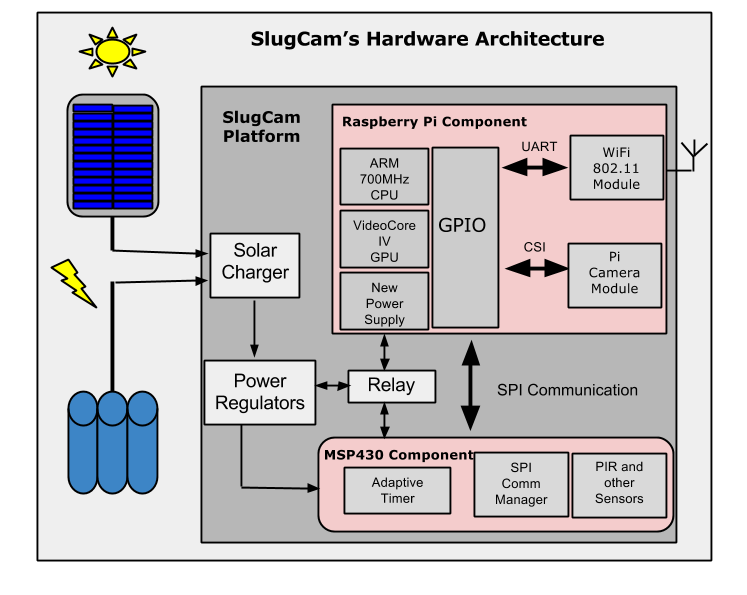
\includegraphics[scale=0.35]{SlugCam_Hardware_Architecture_Diagram.png}
\caption{SlugCam's Hardware Architecture. }
\end{figure}	


\section{Platform Hardware Description}

\subsection{ Node Platform Architecture} (Include a hardware diagram here)
At the core of SlugCam is the Raspberry Pi, an open-hardware device intended to be used by the educational and research community. We have install our own custom embedded linux distro to optimize its performance and processing speeds using the Buildroot tool \cite{buildroot}. Buildroot allows users to cross compile an embedded Linux operating system to fit the needs of an application. Last year the Raspberry Pi Foundation also released an advance camera module that communicates to the pi using the on board CSI interface. The camera supports the ability to take high resolution (2592 x 1944 pixels) images and capture 1080p video at 30 frames per second \cite{rpicamera}. We believe coupling this device with the installed computer vision libraries makes SlugCam attractive to researchers, and has allowed us to use it in monitoring applications requiring accuracy. Just recently we've upgraded to the latest raspberry Pi B+ revision for its power consumption benefits and we later show its beneficial energy efficiency characteristics through experimentation.

\subsection{ The Low Power Control Unit}
With the ability to run on .05$\mu$A during standby and nearly 5 times less then that when sleeping, the MSP430 is the perfect micro-controller to use in a battery reliant node. The MSP430 can decide how long the power hungry Raspberry Pi and its peripherals stay on using a on board timer and an external relay acting as a switch. The Raspberry Pi can dynamically change how much time remains by communicating to the MSP430 over a serial SPI connection.  When SlugCam is in a very low powered sleep state, any external sensor can wake up SlugCam using a hardware interrupt. SlugCam is a multimodal smart camera that uses a passive infrared sensor to decide when to wake up the system, and PIR sensors have been used and studied extensively in other smart camera systems \cite{solarpirvideo}. This sensor fusion technique can use a wide variety of sensors such as an audio sensor like the one the Citric Platform uses \cite{Citric}. WiFi 802.11 has proven to be the most Ubiquitous wireless communication protocol and recently there have been energy efficient modules that have been development for embedded applications. SlugCam uses the RN-171 which is energy efficient and can be put into a low powered sleep state when not in use \cite{wifi}. The MSP430 also records live current consumption data to be processed by SlugCam, allowing it to be a more power-aware system, and to adapt to what battery charge remains.

\subsection{Daughter Card} (may be excluded if not finished in time)

SlugCam also has a custom PCB board that we have created with the external devices and expansive ports to the systems available I/O, and also plugs directly into the Raspberry Pi. The daughter-card improves robustness and reliability, and we provide the the design files on our website. The card also gives SlugCam a more compact size and is less prone to hardware disconnects of external devices in an outdoor environment. Future revisions of SlugCam's daughter-card will have more power efficient wireless modules and sensors for a wider range of outdoor monitoring applications.

\subsection{solar/battery}

Discuss the choice of choosing a solar harvester as an energy source

Mention briefly our research in solar radiation for our area and how solar would not be the best choice everywhere

talk about the choice of the panel and its size

The choice of the battery

Its larger size than needed in order to account for lengthy cloudy periods 

Lithium Ion and our battery technology 

\subsection{The solar charger chip}

Allows for battery health monitoring

charge level features

temperature monitoring for the battery

\subsection{The voltage regulator chip }(optional)




%%
%% *********************  Section 5 **********************************
%%



\section{Software system}

	\subsection{Birds-Eye view of entire system/Overview}
		-Define terms used to describe the rest of system
	\subsection{Node Operating system}
		\subsubsection{Embedded design}
		-Discuss the buildroot tool
		\subsubsection{Power awareness}
The duty cycle discussion
		\subsubsection{OpenCV}

Talk about the popularity of OpenCV in Computer vision applications

Mention our use in being able to detect human objects

more features?
	\subsection{Web Server Stack}
Module design overview (separation of responsibilities into different servers)

Architecture diagram

Workflow diagram

Each module could be swapped out by respecting clearly defined interfaces, so modifications could be easily made after testing and for extensions to the system.

Data Storage Systems (for both discuss reasoning for choices and how we could easily swap for new methods of persistence)

Videos

Message Data

Message Server

Protocol used message transmission

Video Server

Current protocol used for video transmission

Plans to support more advanced video transmission protocol

API Server

Discuss decisions on API design

Easily extensible for future applications

	\subsection{Client Software}
    
Technology choices

Will interface with API server we are designing, can act as an example of how to use API for future developers

Can leverage mobile technologies and still be usable on desktop

Desktop wrapper techniques

Mobile GPS

Description of video file management system

Discussion of querying techniques and how we try to present a large amount of data in a cohesive manner

Maps

Filters



%%
%% *********************  Section 6 **********************************
%%
 
 
 
\section{Deployment} 
	\subsection{ Outdoor power characterization and testing}
    	\subsubsection{experiments in lab with current sensor/multi-meter analyzing the systems current consumption}
		
        \subsubsection{application use cases, both solar/battery performance tests and computer vision tests.}
        
		\subsubsection{solar/battery after}
        
    \subsection{ UI application testing}
    
    
    
%%
%% *********************  Section 7 **********************************
%%    



\section{Background and related work}



%%
%% *********************  Section 8 **********************************
%% 



\section{future work and conclusion}



%% *************************  END PAPER **********************************



% use section* for acknowledgements
\section*{Acknowledgment}


The authors would like to thank...


% Can use something like this to put references on a page
% by themselves when using endfloat and the captionsoff option.
\ifCLASSOPTIONcaptionsoff
  \newpage
\fi



%% ******************  REFERENCE SECTION **********************************



\bibliography{Bib.bib}{}
\bibliographystyle{unsrt}



%% ******************  AUTHOR BIOGRAPHIES *********************************




\begin{IEEEbiographynophoto}{Kevin Abas}
Biography text here.
\end{IEEEbiographynophoto}

\begin{IEEEbiographynophoto}{Leland Miller}
Biography text here.
\end{IEEEbiographynophoto}

\begin{IEEEbiographynophoto}{Katia Obraczka}
Biography text here.
\end{IEEEbiographynophoto}

% You can push biographies down or up by placing
% a \vfill before or after them. The appropriate
% use of \vfill depends on what kind of text is
% on the last page and whether or not the columns
% are being equalized.

%\vfill

% Can be used to pull up biographies so that the bottom of the last one
% is flush with the other column.
%\enlargethispage{-5in}




\end{document}

